\chapter{Motivic Recognition}
\thispagestyle{empty}

\label{motrec}
{\texttt{2015} -- \texttt{2020}}

\bigskip
\smallskip

\section{Introduction}
This article aims to propose an indexing method by estimate the amount of change or variation between two profiles according to a common motive. The profiles in question are symbolic in the sense that the numerical values can refer to any kind of data as melody, dynamic, along with others but in time which is expressed in terms of ordered durations -- such as the formatting of the MDS described in the chapter \textsl{\nameref{mds}}. This approach focuses on the common rhythmic structure in relation to the first derivative applied to it.

The originality of the current approach in the case of a melodic line is to consider its profile only on the sync onsets in order to elude any kind of melodic variations as `\textit{note de passage}', `\textit{monnayage}', `\textit{\'{e}chapp\'{e}e}', `\textit{broderie}', etc.

\bigskip

This work does not take into account the cognitive capacity of the listener or any database, neither music experts evaluation because there is no consensus within the musicologist communities to estimate the proximity of two melodic snippets, at least in terms of relevant parameters, excepts for traditional folk music for which the similarity focuses on tonalities (as interval ratio, ranking notes according to the tone, etc.) and/or rhythm in terms of downbeat among others, raising the quantization problem \citep{desqz} in some non-trivial case. Indeed, for instance two `identical' melodies -- that is to say the same pitches and the same rhythm -- can be perceived very differently according to their respective articulation, tempo and context. And \textit{a contrario}, the feeling of two snippets expressed very differently -- in terms of the opposition of timbres, ornamentation, rhythmic subdivisions, harmonic substitution, and so -- can sound very close, even seen as the same basic melody \citep{hfra}. The border between family resemblance and difference -- even `\textit{diff\'{e}rance}'\citep{dlg}\footnote{This concept fits into the Derrida's deconstruction and plays with on one hand the french homophony `\textit{diff\'{e}rence}/\textit{diff\'{e}rance}' referring in broader terms to an ontological difference and in another hand the polysemy of the french word `\textit{diff\'{e}rer}' (deferral in English) in which reality can only be understood as differential gaps hidden in cultural heritage in space and in time, leaving out or postponing any kind of `re-construction' or conclusion as an open problem.} -- is at the least blurry.

\bigskip

This proposition assumes its own bias and aims to be useful in certain circumstances, notably in the context of \textsl{Neuromuse3} in order to recognize snippets as input sequences and interact knowingly. This algorithm is therefore part of the package N3 -- from version 3.0.9 -- and hence is coded in Common Lisp language. 

\bigskip

Also, this can be an interesting analytical tool in statistical terms applied to a corpus and thus articulate results through a minimal spanning tree as compositional spaces \citep{deec} to that corpus.

\section{Description}

The main function \texttt{differential-vector} is an `experimental' proposition allowing to estimate numerically the distance in terms of motivic proximity between two sequences. This distance is defined according to the cartesian coordinate system as a two-dimensional vector i.e. two criteria defined on the x-axis by the events concordance in relation with the length of the sequences in time as a motive and on the y-axis defined by this motivic profile concordance in terms of signs of the first derivative. 

\bigskip

This implies some algorithmic processes that can be described as follow  (note that all keys described below can be parameterised from the main function \texttt{differential-vector} and the uppercase words refer to functions as subprocesses):

\begin{enumerate}[label= \Alph* --]
\item \myuline{Evaluating $x$}.
\begin{enumerate}

\item Computation of the coordinate $x$ with the functions:

\begin{description}[font=\ttfamily,style=nextline]
\item[\colorbox{gray!20}{DUR->ONSET}] Convert normalised ordered durations to onsets in time for each sequence according to one of the following modalities:
\begin{description}[font=\ttfamily,style=nextline]
\item[\colorbox{gray!20}{:ended :ignore}] set by default, the last duration is ignored;
\item[\colorbox{gray!20}{:ended :first}] the last duration is taken into account as a cyclic pattern;
\item[\colorbox{gray!20}{:ended :last}] the last duration is taken into account with the first derivative equal to zero.
\end{description}

\item[\colorbox{gray!20}{SUBSEQ-THRES}]
Match events  from one sequence to the other according to a given threshold -- key \texttt{\colorbox{gray!20}{:thres}} -- applied as a percentage of the minimal duration of the sequences involved (0.2 by default ).

\item[\colorbox{gray!20}{FILTERNOWAY}] 
Remove if needed onset duplicates on adjacent clusters.
\end{description}

\item Get the percentage of the timing concordance according to the keys:
\begin{description}[font=\ttfamily,style=nextline]
\item[\colorbox{gray!20}{:opt :mean}] set by default, divided the number of concordance by the average of cardinals of the two sequences;
\item[\colorbox{gray!20}{:opt :max}] divided the number of concordance by the maximal cardinal of the two sequences;
\item[\colorbox{gray!20}{:opt :min}] divided the number of concordance by the minimal cardinal of the two sequences.
\end{description}
\end{enumerate}

\item \myuline{Evaluating $y$}.
\begin{enumerate}

\item Computation of the coordinate $y$ according to the rhythmic motive by associating for each selected onset their respective event values, then the function:
\begin{description}[font=\ttfamily,style=nextline]
\item[\colorbox{gray!20}{LX->DX}] compute the first derivative of the motive by sequence according to the `dominant value' of each cluster defining the motive estimated through the keys:
\begin{description}[font=\ttfamily,style=nextline]
\item[\colorbox{gray!20}{:cluster :median}] set by default, retains the mean value of the bigger group in terms of first derivative signs (in case of equality this is the mean value of the union of these groups);
\item[\colorbox{gray!20}{:cluster :mean}] retains the mean value of the cluster;
\item[\colorbox{gray!20}{:cluster :maxima}] retains the maximal value of the cluster;
\item[\colorbox{gray!20}{:cluster :minima}] retains the minimal value of the cluster.
\end{description}
\end{description}

\item Convert the first derivative as signs:
\begin{description}[font=\ttfamily,style=nextline]
\item[$+1$] positive slope,
\item[$-1$] negative slope,
\item[$\ 0$] no slope;
\end{description}

\item apply tolerance if set to \texttt{\colorbox{gray!20}{:yes}} (\texttt{\colorbox{gray!20}{:no}} by default) -- that is to say the values $+1$ and $0$ or $-1$ and $0$ counts as common values;

\item count the common signs of the motives and get the mean value.

\end{enumerate}
\item Values of the output (\texttt{\colorbox{gray!20}{:diff}} as the level of difference, \texttt{\colorbox{gray!20}{:sim}} as the level of similarity, \texttt{\colorbox{gray!20}{-norm}} as the normalised euclidean norm of the vector, \texttt{\colorbox{gray!20}{-coord}} as the coordinate vector and \texttt{\colorbox{gray!20}{-list}} the norm with $x$ and $y$):

\begin{description}[font=\ttfamily]
\item[\colorbox{gray!20}{:result :diff-norm}] (set by default) \\$\displaystyle\frac{\sqrt{(1-x)^2 + (1-y)^2}}{\sqrt{2}}$
\item[\colorbox{gray!20}{:result :diff-coord}] \hfill \\($(1-x)$ $(1-y)$)
\item[\colorbox{gray!20}{:result :sim-norm}] \hfill \\ $\displaystyle\frac{\sqrt{x^2 + y^2}}{\sqrt{2}}$
\item[\colorbox{gray!20}{:result :sim-coord}] \hfill \\ ($x$ $y$)
\end{description}

\end{enumerate}

\section{Evaluation}

Let the following trivial example in figure \ref{fig:dtb} be an illustration of the behaviour of the algorithm, notably the different possible evaluations in relation with the length of the sequences (key \texttt{:opt}) and the result in terms of proximity (key \texttt{:result}).

\begin{figure}[!hbt]
	\begin{center}
		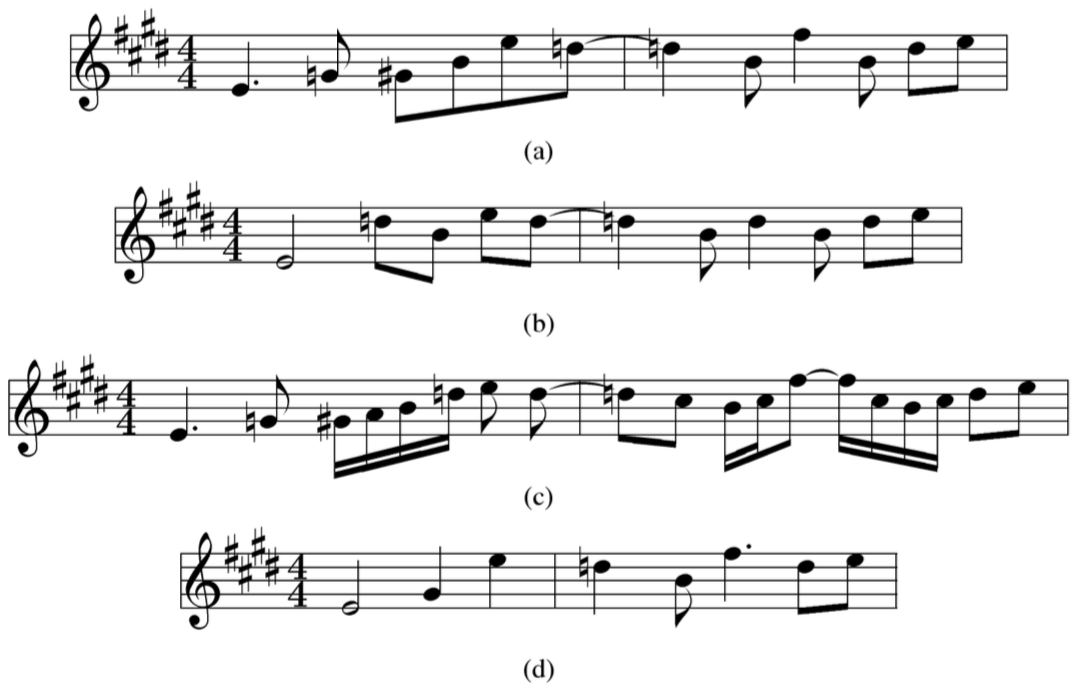
\includegraphics[scale=0.28]{img/8800}
		\caption{(a) Theme of The Beatles' song \textit{Day Tripper} (b) Variation with same tonic \textsf{E} and same dominant \textsf{B} as \textsf{Em} tone (c) Variation with `\textit{notes de passage}' (d) Variation same notes on downbeats \citep[ p. 115]{hfra}.}
		\label{fig:dtb}
	\end{center}
\end{figure}

Let the tables \ref{table:mrdiff} and \ref{table:mrsim} be the results of the function \texttt{differential-vector} as the semi-matrix of distances applied to the four snippets of figure \ref{fig:dtb}, such as the first number of each cell is the percentage of similarity or difference followed by the coordinate vector between square brackets (rounded to two decimal places).

\begin{table}[h!]
\centering
{\ttfamily
\begin{tabular}{|c|r|r|r|}
\hline
\textbf{:diff} & \textbf{:opt :min}        & \textbf{:opt :max}        & \textbf{:opt :mean}       \\
ab    & 08 [0.00 - 0.11] & 10 [0.09 - 0.11] & 09 [0.05 - 0.11] \\
ac    & 00 [0.00 - 0.00] & 25 [0.35 - 0.00] & 15 [0.21 - 0.00] \\
ad    & 09 [0.12 - 0.00] & 26 [0.36 - 0.00] & 19 [0.26 - 0.00] \\
bc    & 08 [0.00 - 0.11] & 30 [0.41 - 0.11] & 20 [0.26 - 0.11] \\
bd    & 00 [0.00 - 0.00] & 14 [0.20 - 0.00] & 08 [0.11 - 0.00] \\
cd    & 09 [0.12 - 0.00] & 42 [0.59 - 0.00] & 31 [0.44 - 0.00] \\
\hline
\end{tabular}}
\caption{Evaluation of the semi-matrix of distances as difference.}
\label{table:mrdiff}
\end{table}

\begin{table}[h!]
\centering
{\ttfamily
\begin{tabular}{|c|r|r|r|}
\hline
\textbf{:sim} & \textbf{:opt :min}        & \textbf{:opt :max}        & \textbf{:opt :mean}       \\
ab  & 95 [1.00 - 0.89]  & 90 [0.91 - 0.89] & 92 [0.95 - 0.89] \\
ac  & 100 [1.00 - 1.00] & 84 [0.65 - 1.00] & 90 [0.79 - 1.00] \\
ad  & 94 [0.88 - 1.00]  & 84 [0.64 - 1.00] & 88 [0.74 - 1.00] \\
bc  & 95 [1.00 - 0.89]  & 75 [0.59 - 0.89] & 82 [0.74 - 0.89] \\
bd  & 100 [1.00 - 1.00] & 91 [0.80 - 1.00] & 95 [0.89 - 1.00] \\
cd  & 94 [0.88 - 1.00]  & 76 [0.41 - 1.00] & 81 [0.56 - 1.00] \\
\hline
\end{tabular}}
\caption{Evaluation of the semi-matrix of distances as similarity.}
\label{table:mrsim}
\end{table}

These tables show a maximal difference of 42\% with the key \texttt{:max} (snippets \texttt{cd} table \ref{table:mrdiff}) and 100\% of similarity with the key \texttt{:min} (snippets \texttt{ac} and \texttt{bd} on table \ref{table:mrsim}).
For the last two cases, that means all notes of the shortest snippet match with the longest and the melodic profile follows the same shape. Knowing that, the key \texttt{:mean} is a good compromise to moderate this bias. 

Also, the \textsf{D}\sh \  of the snippet (d) does not match with others because of the delay of the onset, and the first \textsf{B} of the snippet (b) disrupt the melodic profile on the snippets (a) and (c) ($y$\texttt{:diff}$=0.11$ and $y$\texttt{:sim}$=0.89$).

Note that difference and similarity as normalised vectors (by dividing the norm of the vector by square root of two) are not complementary values in that sense their sum is not always equal to 100\%. More specifically, when the absolute value of $x$ minus $y$ tends toward one, then the summation of the normalised norm of the vectors, respectively as the difference distance $D$ and as the similarity distance $S$, tends toward the square root of two:
$$\text{if } |x-y| \to 1 \text{ then } \frac{||\overrightarrow{D}||}{\sqrt{2}} + \frac{||\overrightarrow{S}||}{\sqrt{2}} \to \sqrt{2}$$
 and furthermore
 $$\text{if } |x-y| \to 0 \text{ then } \frac{||\overrightarrow{D}||}{\sqrt{2}} + \frac{||\overrightarrow{S}||}{\sqrt{2}} \to 1$$
 
 \subsection{Corpus}
 
 In this chapter, the function \texttt{differential-vector} will be applied on the corpus composed of the \textit{fuga} subjects of the first book of the Well-Tempered Clavier (noted WTC I) by Johann Sebastian Bach -- see appendix \fullref{wtc1}.

\smallskip

A note about the corpus; for convenience, every score snippet has been rewritten -- I should say recoded -- in order to elude all articulations and rests since we do not need this information. Concerning the rests it is about to remove them when they are at the head of the melody or to prolong the previous note by adding both durations -- this led to the Lilypond code on the top of each cell of the corpus -- see code in appendix \fullref{code:corpus} in order to generate scores, midi-files and MDS. This is done upstream but this can be done downstream, for instance by filtering the require data on the MDS by keeping pitch durations on their respective onsets in time. 

\smallskip

Also, in the case of the \textit{fuga} subjects, it might appear some unexpected truncation, but sometimes one has to take a side about where the subject stops and when can one considers some `tail' as either a variation, an articulation, a punctuation or a transition. Thus, the problematic raised by the corpus in terms of tails is partially solved by eluding it.

\subsection{Results}

{\color{red}[ ONGOING REVISION ]}

\section{Discussion}

The relevance is relative but this algorithm -- like others -- gives some guidelines in paradigmatic terms as family likeness focusing on the event onsets sync \myuline{proportionally} and on the first derivative \myuline{profile} as the sign values. 

\bigskip

Also, one of the possible applications of this motivic research for a given sequence allows -- according to a given number of events as a pattern or directly a given pattern -- to evaluate sequentially the amount and the relevance of redundancy of this pattern through the considered sequence until this sequence as the whole. Thus, this method can detect all `fractality' in the sequence for a deliberate pattern.
